% Modelo criado por Chaiane Bitelo para o Simpósio de Pós-Graduação em Design do PPDESDI - UERJ
% jun/2020 - Versão 1


\documentclass[a4paper,11pt,oneside,onecolumn,final]{article}

% Estrutura base do documento
% Versão 1
% Desenvolvido por Chaiane Bitelo (PPDEsdi/UERJ)

\usepackage[brazil]{babel}  % adequação para o português Brasil
%\usepackage[utf8]{inputenc} % Determina a codificação utilizada
                            % (conversão automática dos acentos)
\usepackage{graphicx}       % Inclusão de gráficos
\usepackage[alf]{abntex2cite} % pacote para citacoes
\usepackage[top=2.5cm,bottom=2.5cm,left=3cm,right=3cm,headsep=1.3cm,a4paper]{geometry}             % Margens da página

\tolerance=1
\emergencystretch=\maxdimen
\hyphenpenalty=10000
\hbadness=10000

\usepackage{lipsum}          % Insere texto de falso, apenas de marcação

% -----
% USO DA FONTE CAMBRIA
% ----
\usepackage{fontspec}
% Cambria
\setromanfont[
BoldFont=cambriab.ttf,
ItalicFont=cambriai.ttf,
BoldItalicFont=cambriai.ttf,
]{cambria.ttc}

% ----

% --- 
% DEFINE O CABEÇALHO E RODAPE 
% ---
\usepackage{fancyhdr}

\pagestyle{fancy}
\setlength{\headheight}{39pt}
\fancyhf{}
%\rhead{}
\lhead{ \textsc{PCS5029 2020}\\
        \textsc{Processamento de Linguagem Natural com Redes Neurais Artificiais}\\
        17 de setembro a 19 de novembro de 2020
}
\lfoot{\textbf{Resumo estendido} – PCS5029 2020}
\renewcommand{\headrulewidth}{0pt} % retira a linha decorativa do cabeçalho
\renewcommand{\footrulewidth}{0pt} % retira a linha decorativa do rodapé

%------------------------------------------------------------



% ----
% TABELAS E FIGURAS
% ----
\usepackage[singlelinecheck=false,skip=3pt]{caption} % alinha a esquerda e reduz o espaço entre a imagem e a legenda
\usepackage[size=footnotesize]{caption} % reduz o tamanho da fonte
\usepackage{caption}

% Pacote para ajustar a primeira linha da tabela em negrito
\usepackage{array}
\newcolumntype{+}{>{\global\let\currentrowstyle\relax}}
\newcolumntype{^}{>{\currentrowstyle}}
\newcommand{\rowstyle}[1]{\gdef\currentrowstyle{#1}%
#1\ignorespaces
}


% ---  
% Pacote de bibliografia
% ---
\usepackage[alf]{abntex2cite}
\addto{\captionsbrazil}{ % para o uso do \usepackage[brazil]{babel}
\renewcommand{\bibname}{Refer\^{e}ncias} % altera o título para Referências substituindo Referências Bibliográficas
}






\begin{document}
\setlength{\parindent}{0pt} % configura a retirada da identação padrão em parágrafos dos documentos do tipo "article" em Latex 

   
\Huge Bank Word Embeddings ptBR

\vspace{10mm} % espaço entre o título e o início do texto


% ------------- AUTOR DO ARTIGO --------------
% mantenha os comandos abaixo comentados em edições onde a avaliação é cega e o nome do autor deve ser retirado. 

\Large Victor Takashi Hayashi
\vspace{5mm} %5mm vertical space
% --------------------------------------------

% ------- ENTRELINHAS E TAMANHO DA FONTE DOS PARÁGRAFOS --------
\renewcommand{\baselinestretch}{1.15} % configura espaçamento entrelinhas nos parágrafos a partir deste ponto
\normalsize
% ---------------------------------------------------------------

O presente documento destina-se à apresentação do Trabalho Final realizado pelo aluno Victor Takashi Hayashi para a disciplina PCS5029 (IMPLEMENTAÇÃO+RELATÓRIO).

O código fonte está disponível no GitHub: \url{https://github.com/vthayashi/BWE}.

O glossário financeiro do banco Central foi utilizado como corpus:  \url{https://www.bcb.gov.br/content/cidadaniafinanceira/documentos_cidadania/biblioteca/glossario_cidadania_financeira.pdf}

\vspace{5mm}

A tarefa de Processamento de Linguagem Natural escolhida foi o cálculo de similaridade entre palavras do domínio específico bancário, e foi utilizada a arquitetura Continuous Bag Of Words como solução.
O problema considerado foi a estimativa de similaridade semântica entre palavras de um domínio específico, o que pode ser interessante para processos de obtenção de conhecimento a partir de textos em linguagem natural (e.g., estruturando o conhecimento presente nestes dados não-estruturados).
O corpus utilizado foi o glossário simplificado de termos financeiros do Banco Central (Bacen) \cite{glossariobacen}.
A arquitetura Continuous Bag Of Words (CBOW) realiza a predição de uma palavra baseada nas palavras de seu contexto \cite{mikolov2013efficient}.
A biblioteca Python gensim \cite{gensim} foi utilizada para o treinamento da rede neural do CBOW.
A biblioteca NLTK \cite{nltk} com suporte para português brasileiro foi utilizada como ferramenta auxiliar para o preprocessamento do texto de entrada, em conjunto com rotinas encontradas em trabalho de word embeddings da literatura \cite{hartmann2017portuguese}.
Foram comparados dois word embeddings de escopo geral para o português, de modelos CBOW e Glove 50 dimensões com o modelo específico desenvolvido CBOW com 100 dimensões na tarefa de similaridade do cosseno entre os \textit{word embeddings} da palavra 'banco' e outras relacionadas ao domínio bancário.
Foram obtidos 10980 tokens e 1462 termos no vocabulário a partir do glossário do Banco Central, o que é um tamanho equivalente ao menor corpus (SARESP) utilizado em trabalho relacionado \cite{hartmann2017portuguese}.
A Figura \ref{figura} é uma visualização 2D (obtida com Principal Component Analysis) dos word embeddings obtidos com o treinamento específico com o glossário do banco central.
Os resultados estão sumarizados na Tabela \ref{tabela}. A similaridade de 5 palavras com a palavra 'banco' dentre 9 foram maiores com o word embedding específico, enquanto o modelo Glove do escopo geral apresentou melhores resultados de similaridade que o CBOW geral.
O experimento indica que o treinamento específico tem potencial de melhorar os resultados do modelo CBOW para cálculo de similaridade entre algumas palavras do domínio específico bancário.

\begin{table}[ht]
\centering
\begin{tabular}{|r|r|r|r|r|}
\hline
\textbf{Palavras} & \textbf{CBOW geral} & \textbf{Glove} & \textbf{CBOW específico} & \textbf{espec.\textgreater{}geral} \\ \hline
valor             & 0.571603      & 0.665027       & 0.695323     & Sim                           \\ \hline
juros             & 0.248311      & 0.629176       & 0.637589     & Sim                           \\ \hline
pagamento         & 0.522324      & 0.652546       & 0.593549     & Não                          \\ \hline
poupança          & 0.220006      & 0.543432       & 0.632208     & Sim                           \\ \hline
dinheiro          & 0.410055      & 0.621486       & 0.623654     & Sim                           \\ \hline
cliente           & 0.472513      & 0.622152       & 0.564684     & Não                          \\ \hline
comprar           & 0.014624      & 0.526575       & 0.580381     & Sim                           \\ \hline
crédito           & 0.482977      & 0.811110       & 0.553456     & Não                          \\ \hline
serviço           & 0.621220      & 0.625766       & 0.458480     & Não                          \\ \hline
\end{tabular}
\caption{Resultados de similaridade entre 'banco' e outras palavras.}
\label{tabela}
\end{table}


\begin{figure}[ht]
    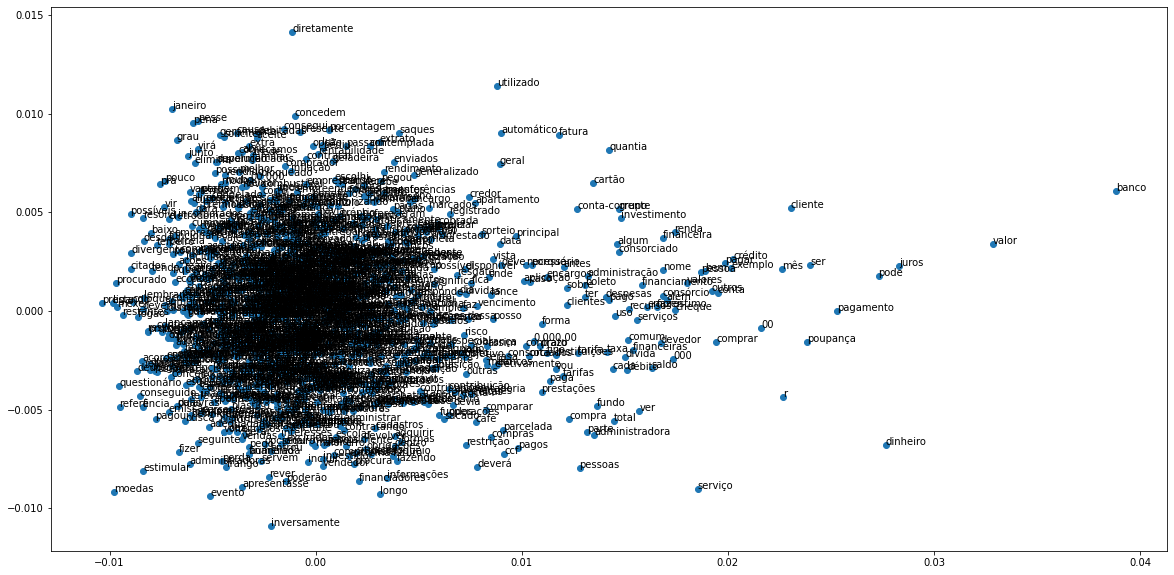
\includegraphics[width=\textwidth]{figura.png} % o tamanho pode ser alterado substituindo o valor em centímetros conforme necessidade. Para a imagem ocupar a mesma largura o texto use o comando \texwidth
    \caption{Visualização 2D obtida com PCA dos word embeddings obtidos.}
    \label{figura}
\end{figure}

\vspace{5mm} %5mm vertical space

\vspace{15mm}

\textbf{Palavras-chave}: Word Embedding. CBOW. Domínio Bancário.


% ---------------
% Referências 
% --------------

\bibliography{bibliografia}



% ------------------------------------
% BIBLIOGRAFIA OCULTA CASO O EDITAL DO ANO CORRENTE TENHA ESSA REGRA
% chama o comando bibliography mas dentro de uma savebox que esconde na hora de compilar o PDF mantendo a execução e garantindo a citação no corpo do texto
%------------------------------------
%\newsavebox\mytempbib
%\savebox\mytempbib{\parbox{\textwidth}{\bibliography{bibliografia}}}
% --------------------------------------


\end{document}
